\documentclass[12pt]{report} % Increased the font size to 12pt
\usepackage{epigraph}
\usepackage{geometry}

% Optional: customize the style of epigraphs
\setlength{\epigraphwidth}{0.5\textwidth} % Adjust the width of the epigraph
\renewcommand{\epigraphflush}{flushright} % Align the epigraph to the right
\renewcommand{\epigraphrule}{0pt} % No horizontal rule
\usepackage[most]{tcolorbox}
\usepackage{amsmath, amssymb, amsthm}
\usepackage{graphicx}
\usepackage{caption}
\usepackage[utf8]{inputenc}
\usepackage{hyperref} % Added for hyperlinks
\usepackage{listings} % Added for code listings
\usepackage{color}    % Added for color definitions
\usepackage[super]{nth} 
\usepackage{fancyhdr}
\usepackage{tikz}
\usetikzlibrary{shapes.geometric, arrows, positioning}

\tikzstyle{startstop} = [rectangle, rounded corners, minimum width=3cm, minimum height=1cm, text centered, draw=black, fill=red!30]
\tikzstyle{io} = [trapezium, trapezium left angle=70, trapezium right angle=110, minimum width=3cm, minimum height=1cm, text centered, draw=black, fill=blue!30]
\tikzstyle{process} = [rectangle, minimum width=3cm, minimum height=1cm, text centered, draw=black, fill=orange!30]
\tikzstyle{decision} = [diamond, minimum width=3cm, minimum height=1cm, text centered, draw=black, fill=green!30]
\tikzstyle{arrow} = [thick,->,>=stealth]

% Define the graphics path
%\graphicspath{{./Plots/}}

% Define the header and footer for general pages
\pagestyle{fancy}
\fancyhf{} % Clear all header and footer fields
\fancyhead{} % Initially, the header is empty
\fancyfoot[C]{\thepage} % Page number at the center of the footer
\renewcommand{\headrulewidth}{0pt} % No header line on the first page of chapters
\renewcommand{\footrulewidth}{0pt} % No footer line

% Define the plain page style for chapter starting pages
\fancypagestyle{plain}{%
  \fancyhf{} % Clear all header and footer fields
  \fancyfoot[C]{\thepage} % Page number at the center of the footer
  \renewcommand{\headrulewidth}{0pt} % No header line
}

% Apply the 'fancy' style to subsequent pages in a chapter
\renewcommand{\chaptermark}[1]{%
  \markboth{\MakeUppercase{#1}}{}%
}

% Redefine the 'plain' style for the first page of chapters
\fancypagestyle{plain}{%
  \fancyhf{}%
  \fancyfoot[C]{\thepage}%
  \renewcommand{\headrulewidth}{0pt}%
}

% Header settings for normal pages (not the first page of a chapter)
\fancyhead[L]{\slshape \nouppercase{\leftmark}} % Chapter title in the header
\renewcommand{\headrulewidth}{0.4pt} % Header line width on normal pages

\setlength{\headheight}{14.49998pt}
\addtolength{\topmargin}{-2.49998pt}
% Define colors for code listings
\definecolor{codegreen}{rgb}{0,0.6,0}
\definecolor{codegray}{rgb}{0.5,0.5,0.5}
\definecolor{codepurple}{rgb}{0.58,0,0.82}
\definecolor{backcolour}{rgb}{0.95,0.95,0.92}

% Setup for code listings
\lstdefinestyle{mystyle}{
    backgroundcolor=\color{backcolour},   
    commentstyle=\color{codegreen},
    keywordstyle=\color{magenta},
    numberstyle=\tiny\color{codegray},
    stringstyle=\color{codepurple},
    basicstyle=\ttfamily\footnotesize,
    breakatwhitespace=false,         
    breaklines=true,                 
    captionpos=b,                    
    keepspaces=true,                 
    numbers=left,                    
    numbersep=5pt,                  
    showspaces=false,                
    showstringspaces=false,
    showtabs=false,                  
    tabsize=2
}

\lstset{style=mystyle}

% Definition of the tcolorbox for definitions
\newtcolorbox{definitionbox}{
  colback=red!5!white,
  colframe=red!75!black,
  colbacktitle=red!85!black,
  title=Definition:,
  fonttitle=\bfseries,
  enhanced,
}

% Definition of the tcolorbox for remarks
\newtcolorbox{remarkbox}{
  colback=blue!5!white,     % Light blue background
  colframe=blue!75!black,   % Darker blue frame
  colbacktitle=blue!85!black, % Even darker blue for the title background
  title=Remark:,            % Title text for remark box
  fonttitle=\bfseries,      % Bold title font
  enhanced,
}

% Definition of the tcolorbox for examples
\newtcolorbox{examplebox}{
  colback=green!5!white,
  colframe=green!75!black,
  colbacktitle=green!85!black,
  title=Example:,
  fonttitle=\bfseries,
  enhanced,
}

% Definitions and examples will be put in these environments
\newenvironment{definition}
    {\begin{definitionbox}}
    {\end{definitionbox}}

\newenvironment{example}
    {\begin{examplebox}}
    {\end{examplebox}}

\geometry{top=1.5in} % Adjust the value as needed
% ----------------------------------------------------------------------------------------

\title{S1 Principles of Data Science Coursework Report}
\author{Thomas Breitburd}
\date{University of Cambridge}

\begin{document} 

\maketitle

\section{Section A}

\subsection*{(a)}

We have the continuous random variable $M \in{[5;5.6]}$. Our model is the weighted sum of a background and signal such that:  


\begin{equation}
p(M;f,\lambda,\mu,\sigma) = fs(M;\mu,\sigma) + (1 - f)b(M;\lambda)
\end{equation}
where:
\begin{center}
$s(M;\mu,\sigma) = \frac{1}{\sqrt{2\pi}\sigma} e^{-\frac{{(M - \mu)}^{2}}{2\sigma^{2}}}$
\end{center}
\begin{center}
$b(M;\lambda) = \lambda e^{-\lambda M}$
\end{center}
\vspace{1\baselineskip}  
We want to show that:  
\begin{equation}
I = \int_{-\infty}^{+\infty} p(M;f,\lambda,\mu,\sigma)\, dM = 1
\end{equation}
We have:  

\vspace{1\baselineskip}  
$I = \displaystyle\int_{-\infty}^{+\infty} fs(M;\mu,\sigma) + (1-f)b(M;\lambda), dM$  

$I = \displaystyle\int_{-\infty}^{+\infty} f\frac{1}{\sqrt{2\pi}\sigma} e^{-\frac{{(M - \mu)}^{2}}{2\sigma^{2}}}\, dM +  \displaystyle\int_{0}^{+\infty} (1-f)\lambda e^{-\lambda M}\, dM$  

\vspace*{1\baselineskip}
Since the exponential decay distribution is only defined from 0 to $+\infty$. We can first evaluate the 2\textsuperscript{nd} integral:  

\vspace*{1\baselineskip}
$\displaystyle \int_{0}^{+\infty} (1-f)\lambda e^{-\lambda M}\, dM  =  (1-f){[-e^{-\lambda M}]}_{0}^{\infty}  =  (1-f)[0 - (-1)]  =  (1-f)$  

\vspace*{1\baselineskip}
Then, we evaluate the integral of the signal part of the model, taking the $f$ weight out. We use a change of variable so that $u = \frac{(M-\mu)}{\sigma} \iff du = \sigma dM$, thus:

\vspace*{1\baselineskip}
$J = \displaystyle \int_{-\infty}^{+\infty} \frac{1}{\sqrt{2\pi}\sigma} e^{-\frac{{(M - \mu)}^{2}}{2\sigma^{2}}}\, dM = \displaystyle \int_{-\infty}^{+\infty} \frac{1}{\sqrt{2\pi}} e^{-\frac{{(u)}^{2}}{2}}\, du$  

\vspace*{1\baselineskip}
We can square multiply this integral by itself, using dummy variables x and y:  

\vspace*{1\baselineskip}
$J^{2} = \displaystyle \int_{-\infty}^{+\infty} \frac{1}{\sqrt{2\pi}} e^{-\frac{{(x)}^{2}}{2}}\, dx \times \displaystyle \int_{-\infty}^{+\infty} \frac{1}{\sqrt{2\pi}} e^{-\frac{{(y)}^{2}}{2}}\, dy$  

$J^{2} = \frac{1}{2\pi}\displaystyle \int_{-\infty}^{+\infty} \int_{-\infty}^{+\infty}  e^{-\frac{{(x)}^{2}}{2}} e^{-\frac{{(y)}^{2}}{2}}\, dx \, dy$  

$J^{2} = \frac{1}{2\pi}\displaystyle \int_{-\infty}^{+\infty} \int_{-\infty}^{+\infty} e^{-\frac{1}{2}(x^{2}+y^{2})}\, dx \, dy$  

\vspace*{1\baselineskip}
From here, we can switch to polar coordinates to be able to evaluate this. We have $x = r\cos{(\theta)} y = r\sin{(\theta)}$. This means we need to change the limits to polar equivalents. We will get $r \in{[0,\infty]}$ and $\theta \in{[0,2\pi]}$. Further, $dx dy = r dr d\theta$:  

\vspace*{1\baselineskip}
$J^{2} = \frac{1}{2\pi}\displaystyle \int_{0}^{2\pi} \int_{0}^{+\infty} e^{-\frac{1}{2}r^{2}}r\, dr \, d\theta$  

$J^{2} = \frac{1}{2\pi}\displaystyle \int_{0}^{2\pi} {[-e^{-\frac{1}{2}r^{2}}]}_{0}^{\infty}\, d\theta$  

$J^{2} = \frac{1}{2\pi}\displaystyle \int_{0}^{2\pi} [-0 - (-1)]\, d\theta$  

$J^{2} = \displaystyle \frac{1}{2\pi}\displaystyle \int_{0}^{2\pi} 1\, d\theta$  

$J^{2} = \displaystyle \frac{1}{2\pi}\displaystyle {[\theta]}_{0}^{2\pi}$  

$J^{2} = \displaystyle \frac{1}{2\pi}\displaystyle {[2\pi - 0]}$  

$J^{2} = 1$ 

\vspace*{1\baselineskip}
This then means that $J = \pm 1$ but since $s(M;\mu,\sigma) > 0 \forall M \in [-\infty,\infty]$, $ J = 1$. Thus: $I = (1-f) + f = 1$.  


\subsection*{(b)}
We want to find an expression of $p(M;\vec{\theta})$ such that it is normalised between $\alpha$ and $\beta$. Now because the signal fraction $f$ is such that:

\begin{equation}
    \frac{s(M;\mu,\sigma)}{b(M;\lambda)} = \frac{f}{1-f}
\end{equation}

This means that we need to normalise the signal and background components separately. This gives:

\begin{equation}
    \displaystyle \int_{\alpha}^{\beta} f N_{s} \times s(M;\mu,\sigma) + (1 - f)N_{b} \times b(M;\lambda)\, dM = 1
\end{equation}  

with:

\begin{equation}
    \frac{1}{N_{s}} = \displaystyle \int_{\alpha}^{\beta} s(M;\mu,\sigma)\, dM
\end{equation}

\begin{equation}
    \frac{1}{N_{b}} = \displaystyle \int_{\alpha}^{\beta} b(M;\lambda)\, dM.
\end{equation}

\vspace*{1\baselineskip}
where $N_{s}$ and $N_{b}$ are a function of parameters $\vec{\theta}$. Now, from the definition of the Cumulative Distribution Function (c.d.f.): $F(X') = \int_{-\inf}^{X'} f(X)\, dX$, where $X'$ is a specific value of the random variable $X$, and $f(X)$ is the p.d.f.(The lower limit is 0 for the exponential decay distribution). This means we can write (5) and (6) as:

\begin{equation}
    \frac{1}{N_{s}} = \displaystyle \int_{\alpha}^{\beta} s(M;\mu,\sigma)\, dM = F_{s}(\beta) - F_{s}(\alpha)
\end{equation}

\begin{equation}
    \frac{1}{N_{b}} = \displaystyle \int_{\alpha}^{\beta} b(M;\lambda)\, dM = F_{b}(\beta) - F_{b}(\alpha)
\end{equation}

\vspace*{1\baselineskip}
We know that the normal and exponential decay distributions have:  

\begin{equation}
    Normal: \displaystyle F(X) = \frac{1}{2}[1 + erf(\frac{X - \mu}{\sigma\sqrt{2}})]
\end{equation}  

\begin{equation}
    Exponential\ Decay: \displaystyle F(X) = 1 - e^{-\lambda X}
\end{equation}  

\vspace*{1\baselineskip}
From equation (7) and (8), we can write the normalisation factors as:

\begin{equation}
    \frac{1}{N_{s}} = \frac{1}{2}[1 + erf(\frac{\beta - \mu}{\sigma\sqrt{2}})] - \frac{1}{2}[1 + erf(\frac{\alpha - \mu}{\sigma\sqrt{2}})] = \frac{1}{2}[erf(\frac{\beta - \mu}{\sigma\sqrt{2}}) - erf(\frac{\alpha - \mu}{\sigma\sqrt{2}})]
\end{equation}

\begin{equation}
    \frac{1}{N_{b}} = (1 - e^{-\lambda \beta}) - (1 - e^{-\lambda \alpha}) = e^{-\lambda \alpha} - e^{-\lambda \beta}
\end{equation}

\vspace*{1\baselineskip}
Finally, this gives the total p.d.f.\ of the model as:

\begin{equation}
    p(M;\vec{\theta}) = \frac{f}{2}[erf(\frac{\beta - \mu}{\sigma\sqrt{2}}) - erf(\frac{\alpha - \mu}{\sigma\sqrt{2}})] \times s(M;\mu,\sigma) + (1 - f)[e^{-\lambda \alpha} - e^{-\lambda \beta}] \times b(M;\lambda)
\end{equation}

\subsection*{(c)}

In this question, we check that the integral of the p.d.f.\ between $\alpha$ and $\beta$ does equal unity. For this specific case, the \texttt{scipy.integrate} library is used to numerically integrate the component-wise normalised p.d.f.\ as described in equation (4). Though $N_{s}$ and $N_{b}$, are computed using the \texttt{scipy.integrate} library, like in (5) and (6). The components are computed using \texttt{scipy.stats} library's \texttt{norm.pdf} and \texttt{expon.pdf} methods (cf.\ \texttt{funcs.py} file, \texttt{pdf\_norm} function). Then, the weighted sum of the two is computed. Finally, that p.d.f.\ is integrated from $\alpha$ to $\beta$, with randomly generated $\vec{\theta}$ parameters, using \texttt{random.uniform}. The results are shown in the table below:

\begin{center}
    \begin{table}[htbp]
        \begin{tabular}{ |c|c|c|c|c| } 
            \hline
            $\mu$ & $\sigma$ & $\lambda$ & $f$ & $Integral$ \\ 
            \hline
            5.2357 & 0.0190 & 0.3643 & 0.5044 & 1.0 \\ 
            \hline
            5.5436 & 0.0105 & 0.3823 & 0.6081 & 1.0 \\ 
            \hline
            5.3184 & 0.0214 & 0.6424 & 0.6882 & 1.0 \\ 
            \hline
            5.3621 & 0.0221 & 0.3695 & 0.3625 & 1.0 \\ 
            \hline
            5.3640 & 0.0231 & 0.5015 & 0.2442 & 1.0 \\ 
            \hline
        \end{tabular}
        \centering
        \caption{Results for different values of $\vec{\theta}$ parameters.\ (cf.\ \texttt{solve\_part\_c.py} file)}
    \end{table}
\end{center}

\subsection*{(d)}

For this question, the true values of the parameters were set and used to plot the p.d.f.\ of the model, along with the signal and background component overlayed. The parameters are assumed to be:

\begin{center}
    $\mu = 5.28$;  
    $\sigma = 0.018$; 
    $\lambda = 0.5$; 
    $f = 0.1$
\end{center}

The \texttt{signal\_norm}, \texttt{background\_norm}, and \texttt{pdf\_norm} functions, described in (c) were used to compute the p.d.f.\ of the model, signal, and background, normalised for $M\in{[5,5.6]}$. The results are shown in the figure below:

\newpage

\begin{figure}[htbp]
    \centering
    \includegraphics[width=\textwidth]{/Users/thomasbreitburd/Documents/CAMBRIDGE/Study/Principles_of_DS/Coursework/tmb76/Plots/plot_pdf_d_comp.png}
    \captionsetup{margin=1.3cm}
    \caption[width=0.2\pdfpagewidth]{Plot of the total p.d.f.\ of the model, signal, and background, normalised for $M\in{[5,5.6]}$.}
\end{figure}  

This shows the impact of the $f$ weight, which considerably reduces the size of the signal component in the total p.d.f.. 

\subsection*{(e)}

The ``true'' p.d.f., signal and background component are now known and have been visualised. The context is now to generate a dataset from this ``true'' p.d.f., and to assume this is an observed sample obtained in an experiment. From this sample, the goal is now to try and estimate these ``true'' parameters, using a chosen estimation method.  

To generate the sample, an accept-reject method was used. The accept-reject method requires us to know the p.d.f.\ function over the $M$ domain, and the maximum value of the p.d.f.\ in the $M$ domain, $y_{\max}$. Uniformly random values of $M$ between $\alpha$ and $\beta$ are generated, using \texttt{random.uniform}. Then, for each of these values, many uniform random values of $y$ are generated between 0 and $y_{\max}$. If these generated $y$'s are such that $y \leq p(M;\vec{\theta})$ for the generated $M$ then the \textbf{$\mathbf{M}$ value} is accepted and added to the sample. This is repeated until the sample size is reached (cf.\ \texttt{funcs.py} file, \texttt{accept\_reject} function).  

The chosen estimation method is the Maximum Likelihood Estimation (MLE) method. This method relies on the likelihood function, which stands for the probability of observing the data given a set of parameters and is defined as:

\begin{equation}
    \mathcal{L}(\vec{\theta}) = \displaystyle \prod_{i=1}^{N} p(M_{i};\vec{\theta})
\end{equation}

It is a function of the parameters $\vec{\theta}$ only. The goal of the MLE method is to find estimates of the parameters $\vec{\theta}$ that maximise the likelihood function. In other words, finding $\vec{\hat{\theta}}$, such that:  

\begin{equation}
    \frac{\delta\mathcal{L}(\vec{\hat{\theta}})}{\delta \theta} = 0
\end{equation}

This result is because maximising the probability of observing $M$ given a certain set $\vec{\hat{\theta}}$ means we have found the set of parameters $\vec{\hat{\theta}}$ that are the most likely to be the ones the data was observed under. Now because summing small numbers is less of a problem as multiplying small numbers in computations, we take the logarithm of the likelihood function, to turn the product into a sum. And taking twice the negative of that gives a negative log-likelihood function:

\begin{equation}
    -2\ln{\mathcal{L}(\vec{\theta})} = -2\displaystyle \sum_{i=1}^{N} \ln{p(M_{i};\vec{\theta})}
\end{equation}

And this is the function to now \textbf{minimise}. To do so we use a python package named \texttt{iminuit}, which possesses a very useful set of minimising tools. The \texttt{iminuit} package requires a function to minimise, called a cost function, and a set of initial guesses for the parameters. Luckily, \texttt{iminuit} possesses a series of standard cost functions. The one used here is the \texttt{BinnedNLL}, Binned Negative Log-Likelihood, which takes in the c.d.f.\ of a \textbf{normalised} probability density and the observed \textbf{binned} data we want to fit that density to. With the cost function defined, \texttt{iminuit}'s main function \texttt{Minuit}, a function minimizer and error computer, takes that cost function in along with initial guesses for the parameters. These initial guesses are usually educated guesses at what the true parameters may be. Then we call the \texttt{migrad} method, which is a gradient descent method, to conduct the minimization.

An important point is that \texttt{iminuit.Minuit} reads the function given in the cost function definition to read the parameters it needs to fit for. In other words, using the \texttt{pdf\_norm} function from (d), \texttt{Minuit.migrad()} would minimise the cost function for the $\vec{\theta}$ parameters as well as $\alpha$ and $\beta$.

Furthermore, in the interest of performance, the \texttt{numba\-stats} library was used to speed up any computation that uses our new p.d.f.\ function. This library provides \texttt{numba}-accelerated statistical function for common probability distributions. So the c.d.f.\ of the model was defined to only take the $\vec{\theta}$ parameters. It then uses the \texttt{numba\_stats.truncnorm.cdf} and \texttt{.truncexpon.cdf} functions. Running the minimisation, the following parameter estimates and their uncertainties were obtained:  

\begin{center}
    $\hat{\mu} = 5.27939 \pm 0.00033$;  

    $\hat{\sigma} = 0.01820 \pm 0.0032$;  
    
    $\hat{\lambda} = 0.490 \pm 0.019$;  

    $\hat{f} = 0.1008 \pm 0.0017$
\end{center}

We can see that the minimisation performed well, with close estimates and relatively small uncertainties. And the following plot of the data and the fitted model was obtained:

\newpage
\begin{figure}[htbp]
    \centering
    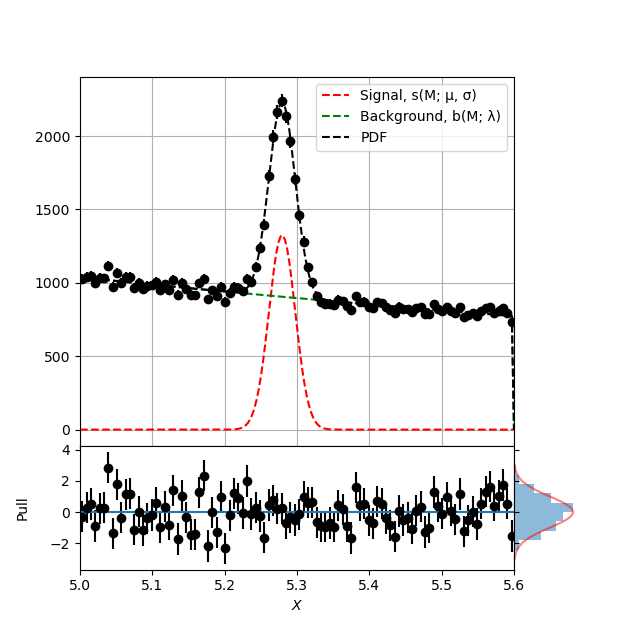
\includegraphics[width=\textwidth]{/Users/thomasbreitburd/Documents/CAMBRIDGE/Study/Principles_of_DS/Coursework/tmb76/Plots/plot_pdf_e.png}
    \captionsetup{margin=1.3cm}
    \caption[width=0.2\pdfpagewidth]{Plot of the data and the fitted model.}
\end{figure}

The lower plots are plots of the pull: $pull = \frac{obs - pred}{\sqrt{N}}$, where $N$ is the bin counts. The pull plots are a good way to check that the uncertainties are sensible. If there were a visible trend in the pull v M plot, or if the pull distribution plot on the right was not normally distributed, then the uncertainties would be too small or too large.




\section{Section B}

blabla

\end{document}
